
\newpage
\newgeometry{left=1.5cm, right=1.5cm, top=0.8cm, bottom=1cm}
\begin{figure}[p]
      \thispagestyle{empty} % Suppress the page number on this page
      \centering
      \captionsetup{justification=centering, labelfont=bf}
      \parbox{\textwidth}{\centering \Huge Healthy derived Network - hSBM       \vspace{0.5cm} } % 
      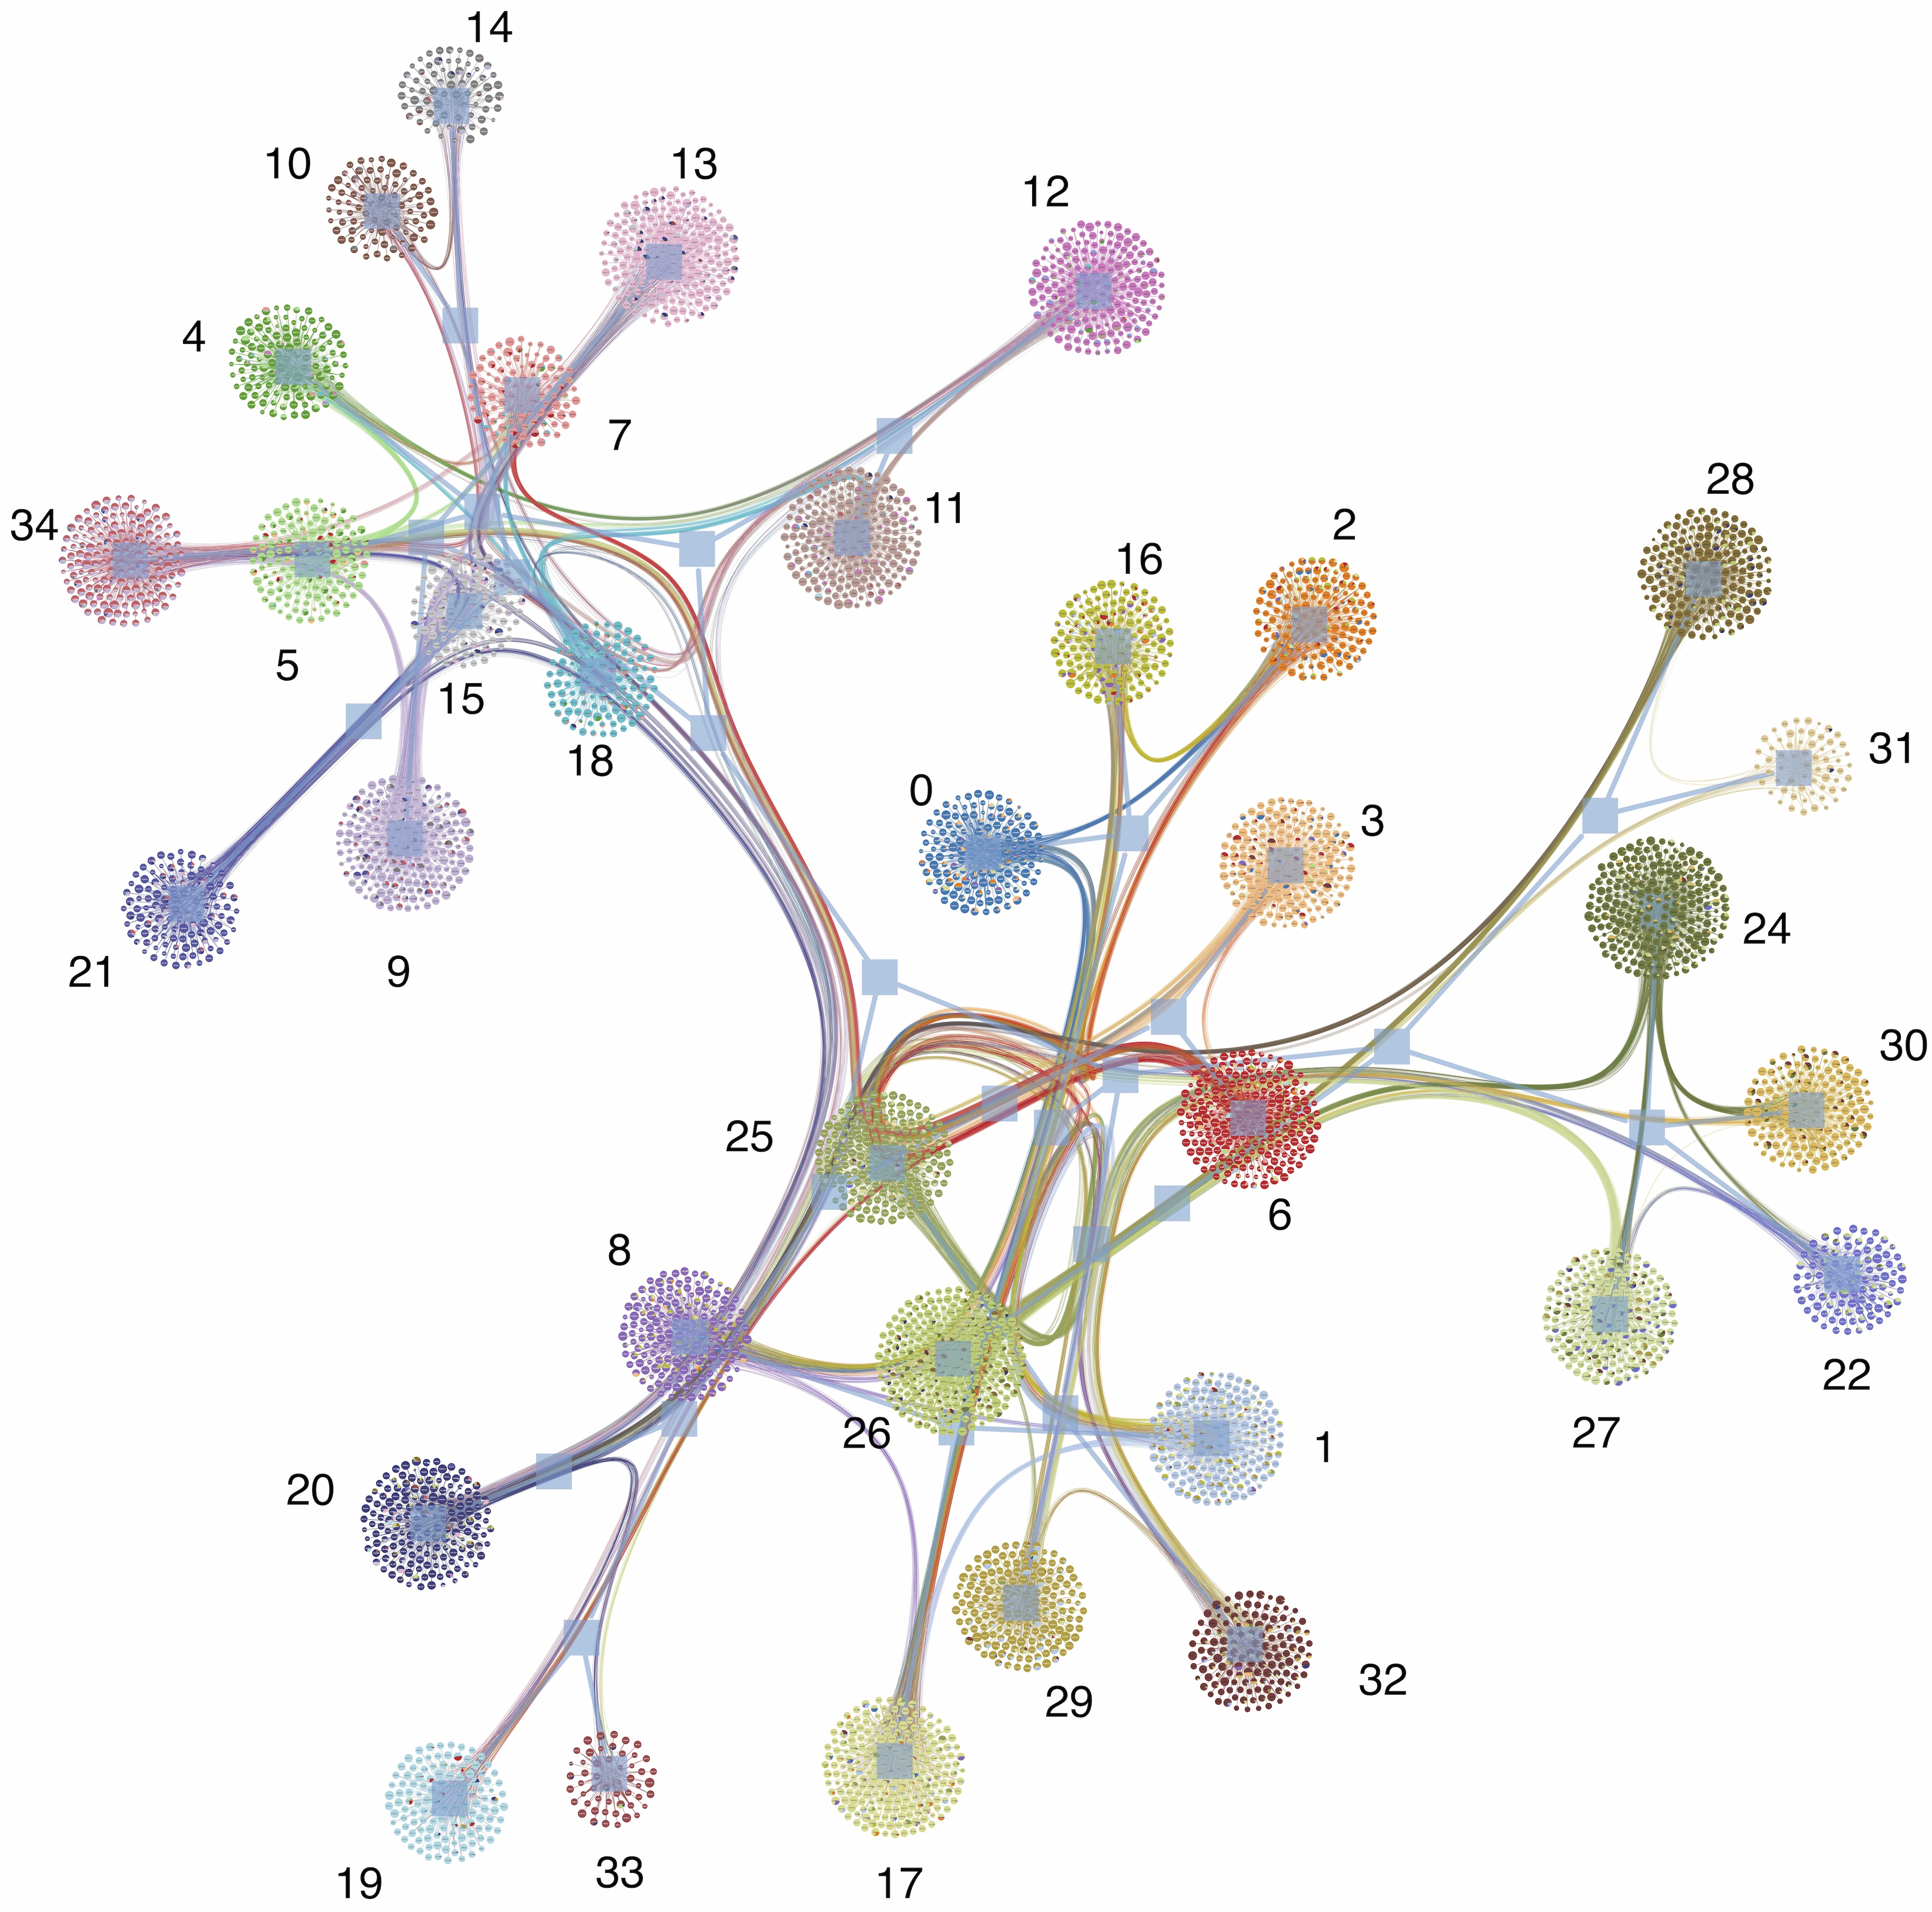
\includegraphics[width=0.9\paperwidth,keepaspectratio]{Sections/Network_pages/images/hier_sfdp_standard_5K_6TF_hsbm_6K_v2_labels_low_res.jpg} 
      \vspace{0.5cm}
      \label{fig:N_II:standard_network}
      \parbox{0.8\textwidth}{Network created using the 5000 most varied genes in the healthy dataset, no weight modifier, minimum degree of 3 for standard genes and 6 for TF. \acrlong{hsbm} is used for community detection algorithm. See \cref{fig:N_II:reward_net} for the network where the mutation are integrated.}
\end{figure}
\restoregeometry
